\chapter{Continuation Methods}\label{ch_cm}
Continuation methods are powerful tools that can be used to find solutions of a parameterized nonlinear system of equations of the form
\begin{align} \label{non_sys}
&\mathbf{G}(\mathbf{x},\alpha) = 0,& & \mathbf{G}: \mathbb{R}^n\times\mathbb{R}^p\rightarrow\mathbb{R}^{n},
\end{align}
where $\mathbf{x} \in \mathbb{R}^{n}$ is a discretized solution of the nonlinear system of $n$-equations and
$\alpha \in \mathbb{R}^p$ are parameters of the system. The solutions  of the nonlinear system of equations~(\ref{non_sys}) are manifolds connected at \emph{singularity} solutions or bifurcation points. In the case of  $p =1$, these manifolds are curves $\Gamma$ that lie in the space $(\mathbf{x},\alpha)$. In practice, such curves are approximated by a set of discrete points $\left\{(\mathbf{x}_i,\alpha_i)\right\}_{i=0}^n$ which correspond to an approximate solutions of the nonlinear system~(\ref{non_sys}), and which can be found using continuation methods. Specifically, assume that an approximate solution $\mathbf{x}_0$ for the nonlinear system~(\ref{non_sys}) is known for parameter value $\alpha = \alpha_0$ i.e. $(\mathbf{x}_0,\alpha_0)$ is a point on $\Gamma$. This point is used to find the next point $(\mathbf{x}_1,\alpha_1)$  on the curve and this new point to find the next, and so on, thus tracing out the curve.

This chapter gives an overview of continuation methods and their application to dynamical systems. In Section~\ref{sc_ti_ap}, we discuss matrix-free methods which are memory-efficient methods that are effective for the application of continuation methods to large-dimensional systems. The application of these methods to detect equilibria and periodic solutions and to identify their local behaviours for the annular electroconvection problem are discussed in Section~\ref{sc_ti_ap} and~\ref{sec_lin_sta_ana}.

\section{Methodology}\label{sc_meth}
In general, continuation methods consist of a two step, predictor-corrector procedure. In the first step a guess $(\hat{\mathbf{x}}_1,\hat{\alpha}_1)$ is predicted by an extrapolation from a known solution $(\mathbf{x}_0,\alpha_0)$ to the nonlinear system~(\ref{non_sys}). In the second step, a nonlinear solver, e.g. of Newton type, is used to correct the guess to within a desired tolerance.

The most common continuation method in the literature is pseudo-arclength continuation~\cite{Con_meth_2,Con_meth_1}, which was introduced by Keller~\cite{Keller} in the late 1970s. In pseudo-arclength continuation, the solution curves $\Gamma$, the state variable $\mathbf{x}$, and a scalar parameter of the nonlinear system $\alpha$ are parameterized using an independent arclength parameter $s$, i.e. $\Gamma(s):= (\mathbf{x}(s),\alpha(s))$. Using this approach, the solution curves are traced out along the arclength parameter $s$. In one type of pseudo-arclength continuation known as the \emph{Keller method}, the nonlinear solver makes the correction along the plane orthogonal to the tangent space of the curve~\cite{Con_meth_1}. This method is desirable for its ability to trace curves that fold back on themselves. At these \emph{fold} points (see Figure~\ref{fig_con_non_sys}), the Jacobian of the nonlinear system~(\ref{non_sys}) with respect to $\mathbf{x}$  becomes singular, leading to problems in the solutions of the linear system obtained using Newton-like solvers which depend mainly on the Jacobian to approximate solutions of~(\ref{non_sys}). For the sheared annular electroconvection problem, we do not anticipate \emph{fold} points. Thus, we choose to implement natural numerical continuation methods in which the solution curves $\Gamma$ are parametrized using the natural parameter $\alpha$ of the nonlinear system, $\Gamma(\alpha):=\left(\mathbf{x}(\alpha),\alpha\right)$. This method makes the correction along the plane orthogonal to the paramater $\alpha$ plane (see Figure~\ref{fig_con_non_sys}), and thus fails at \emph{fold} points. The benefit of natural continuation is that it is slightly easier to implement then pseudo-arclength continuation.
\begin{figure}[t]
\centerline{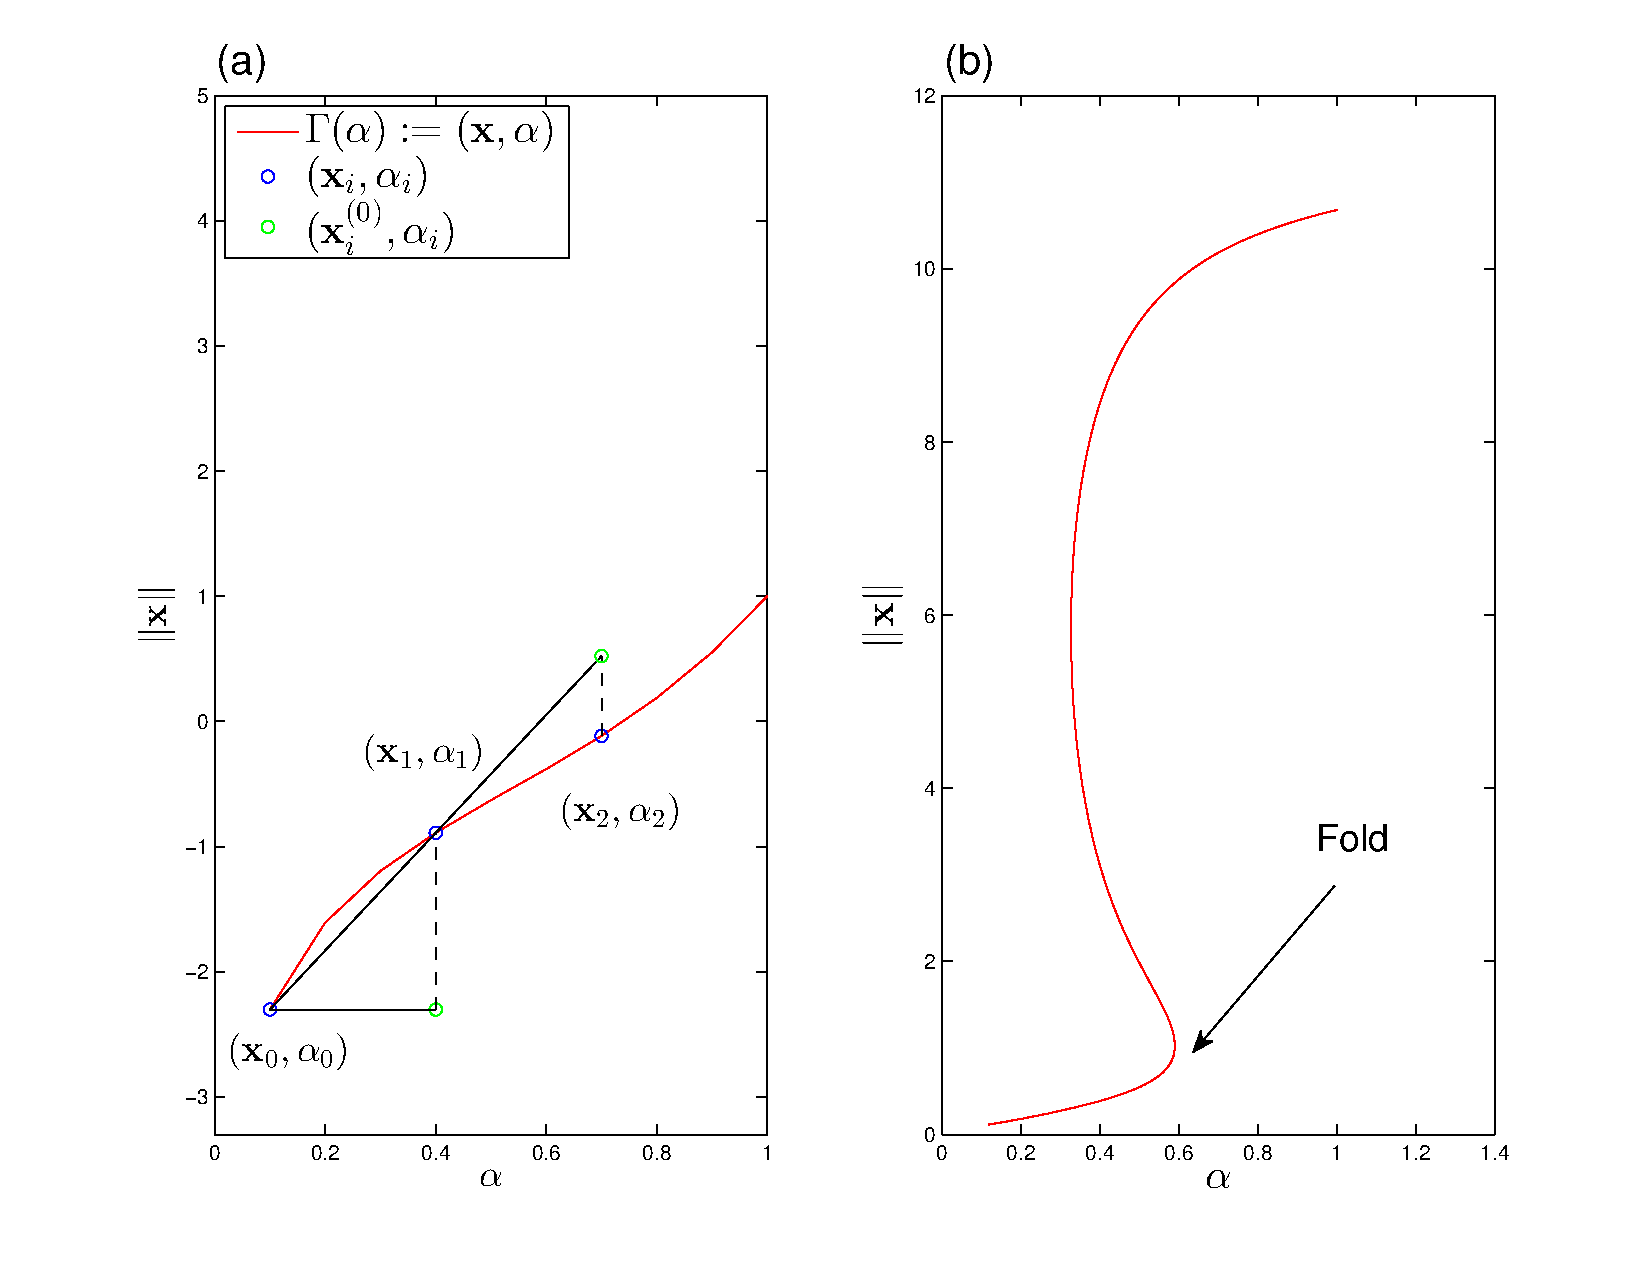
\includegraphics[ width = 1.1\textwidth]{./figures/Pictures/Ill_Nat_CM.pdf}}
\caption{The natural continuation method with a secant extrapolation. The solution points on the curve are represented by $(\mathbf{x}_i,\alpha_i)$, the vertical axis represents some norm of the state vector $\mathbf{x}$ and the horizontal axis represents the parameter of the nonlinear system $\alpha$.}
\label{fig_con_non_sys}
%[Illustration of the natural continuation method with a secant extrapolation]
\end{figure}

The methodology of the natural continuation method  is illustrated in Figure~\ref{fig_con_non_sys}. In the first step, a guess $(\mathbf{x}_{i+1}^{(0)},\alpha_{i+1})$ is generated by an extrapolation  along a secant line from the previously computed solutions $(\mathbf{x}_{i},\alpha_{i})$ :
\begin{align}
& \alpha_{i+1} = \alpha_i + \delta,  && i \ge 0,\\
&\mathbf{x}_{i+1}^{(0)} = \mathbf{x}_{i},  && i = 0,     &&\\
&\mathbf{x}_{i+1}^{(0)} = \mathbf{x}_{i} + \frac{\mathbf{T}}{\|\mathbf{T}\|_2} \delta,  && i \geq 1,  && \mathbf{T} = \mathbf{x}_{i}-\mathbf{x}_{i-1}.
\end{align}
Here, the subscript $i$ denotes the point on the curve, the superscript denotes the number of nonlinear solver iterations and $\delta$ is a small increment step of the parameter $\alpha$.
In the second step, a Newton-Raphson solver can be used to refine the guess to within a given tolerance along the plane orthogonal to the axis of the parameter $\alpha$, i.e. for which $\alpha$ is constant. Specifically the iterate $\mathbf{x}_{i}^{(k+1)}$ can be found from the following linear equation
\begin{subequations}\begin{align}
\mathrm{D}_{\mathbf{x}}\mathbf{G}(\mathbf{x}_{i}^{(k)},\alpha_i)\delta \mathbf{x} &= -\mathbf{G}(\mathbf{x}_{i}^{(k)},\alpha_i),\\
\mathbf{x}_{i}^{(k+1)} &=\mathbf{x}_{i}^{(k)} + \delta \mathbf{x},
\end{align}\end{subequations}
where $\mathrm{D}_{\mathbf{x}}\mathbf{G}$ is the Jacobian of $\mathbf{G}$ with respect of $\mathbf{x}$ and $\delta{\mathbf{x}}$ is a Newton correction.
%Although the natural continuation methods is easier to implement than the pseudo-arclength, it fails to trace folds (see Figure~\ref{fig_con_non_sys}). At this fold points, the Jacobian of the nonlinear system $\mathrm{D}_{\mathbf{x}}\mathbf{G}(\mathbf{x},\alpha)$ becomes singular. In this case, pseudo-arclength continuation (see \cite{Con_meth_2}, \cite{Con_meth_1}), in which the nonlinear solver makes the correction along the plane orthogonal to the tangent space of the curve, is the appropriate choice. However, we do not anticipate folds, therefore we choose to implement a numerical natural continuation method.
%The solution points on the curve are represented by $\mathbf{X}_i = (\mathbf{x}_i,\alpha_i)$, the yaxis represents some norm of the state vector $\mathbf{x}$ and the xaxis represents the parameter of the nonlinear system $\alpha$.
%
%The pseudo-arclength methods have advantages on the natural continuation methods which fails to trace the solution curves around folds. In the pseudo-arc ince it traces the solution curves even around folds where the Jacobian of the nonlinear system becomes singular. In the pseudo-arclength, the
%%This type of parametrization is known as the natural parametrization.
%...
%We implement the numerical natural continuation method from scratch in MATLAB. We choose a secant extrapolation to predict the guess and Newton-Raphson nonlinear solver to correct the guess to the solution.
%%In the natural parametrization, the solution curve we denote $\Gamma$ is parametrized using the nonlinear system parameter $\alpha$.
%In the predictor step, starting from the known solution $(\mathbf{x}_0,\alpha_0)$, we choose the guess point $(\hat{\mathbf{x}}_1,\hat{\alpha}_1)$ such that,
%\begin{equation*}\begin{split}  \hat{\mathbf{x}}_1 = \mathbf{x}_0\\ \hat{\alpha}_1 = \alpha_0 + \delta, \end{split}\end{equation*} where $\delta$ is a step size, and then
\section{Application to Dynamical Systems}\label{sc_app}
One of the applications of continuation methods is to detect and compute invariant limit sets, such as steady states, limit cycles and invariant tori, of continuous dynamical systems of the form
\begin{align}
\label{dyn_sys}
&\deriv[]{}{t}\mathbf{u} = \mathbf{f}(\mathbf{u},\mu),& & \mathbf{f}: \mathbb{R}^n\times\mathbb{R}^p\rightarrow\mathbb{R}^n,
\end{align}
where $\mathbf{u}:=\mathbf{u}(t) \in \mathbb{R}^n$ is a state variable of the dynamical system and $\mu \in \mathbb{R}^p$ are the parameters of the system.  Upon obtaining these invariant limit sets, one can investigate their local behaviours, e.g. using linear stability analysis, and in the process, identify bifurcation points. The aim is to find representations (qualitative and quantitative) of the different types of behaviour that the system may exhibit depending on key parameters. The results can then be summarized in a bifurcation diagram, wherein the parameter space is partitioned into regions of topologically different behaviour.

Many fluid problems, such as annular electroconvection are modelled  by a set of partial differential equations (PDEs), along with algebraic equations (AEs) obtained from conservation laws and modelling approximations. By implementing for example a streamfunction-vorticity formulation, then discretizing the spatial variables using  a spectral, finite-difference, or finite-element method, the set of PDEs and AEs can be written as a continuous dynamical system in the general form
\begin{align}
\label{eq_gen_dy_sys}
&\mathcal{M}\deriv[]{}{t}\vec{u} = \vec{F}(\vec{u},\mu) = \mathcal{L}\vec{u} +\mathcal{N}(\vec{u}), &
&\mathbf{F}: \mathbb{R}^n\times\mathbb{R}^p\rightarrow\mathbb{R}^n,
\end{align}
where $\mathcal{M}$ is the mass matrix, typically not invertible due to algebraic constraints, $\mathcal{L}$ is a linear operator, $\mathcal{N}(\vec{u})$ is a nonlinear operator, and $\mathbf{u}=\mathbf{u}(t) \in \mathbb{R}^n$ is the discretized solution of the governing equations. In general, the size $n$ of the solution vector $\mathbf{u}$  is determined by
the number of the dynamic physical quantities that are modelled, and the size of the discretization (which is dependent on the dimension of the physical system). In the case of annular electroconvection considered in this thesis, the solution vector $\mathbf{u}$ is composed of four 2D physical quantities (the electric potential $\psi_2$, the charge density $q$, the vorticity $\omega$, and the streamfunction $\phi$) that are discretized using spectral methods on the domain. Thus, the size of the vector $\mathbf{u}$ is $n = 4(2K+1)(N_c+1)$,  where $K$ is the highest Fourier mode and $N_c$ is the highest degree of Tchebychev polynomial as shown in Chapter 2.

In many fluid applications, one is interested in the changes in the long-time solutions of~(\ref{eq_gen_dy_sys}) as parameters are varied. For example in the case of sheared annular electroconvection, transition in the flow occurs due to a change in the applied voltage. In dynamical system theory, regardless of the initial state, the system will approach solutions known as attractors of~(\ref{eq_gen_dy_sys}) after sufficiently long time. The simplest attractor of a model is a steady state. Other type of attractors, in order of increasing complexity, are limit cycles, invariant tori and chaotic attractors. Transition between attractors occurs through bifurcations as parameters are varied. The type of bifurcation can be classified from its normal form, which is a simplified system of ordinary differential equations (ODEs); For details see any introductory book of Dynamical Systems; e.g.~\cite{strogatz2014}.

Numerical time-integration is often used to find these attractors and transition behaviours of the system, i.e. parameters are successively changed and the asymptotic behaviour is studied by observing the evolution of the initial value problem. The practicality of this approach is favourable for the identification of chaotic attractors. However, for classification of the behaviours of these attractors as a function of parameters, numerical bifurcation methods are the preferred choice due to the systematic and efficient approach in the computation of attractors and bifurcation points.
In some cases, the local behaviour of such attractors may be identified using linear stability analysis.

In 1979, Eusebius J. Doedel implemented a software package called AUTO, which performs an automated bifurcation analysis. AUTO has become the most widely used software for bifurcation analysis. However, although AUTO performs well for algebraic systems and ODEs~\cite{Doedel_auto2000}, its methods are not designed for large-scale problems such as sheared annular electroconvection. Therefore in this thesis, we do not use AUTO but instead choose to implement a numerical bifurcation method that uses a different approach in computing steady states and limit cycles. %In particular, we are concerned with both steady states and limit cycles.
In Section~\ref{sc_st_ap}, we first present examples of methods used in AUTO, which we refer to as the standard approach, and discuss the challenges that occur when applying such methods to large-scale problems. Some of these challenges can be overcome by instead implementing a set of techniques based on time-integration; see Section~\ref{sc_cha_diff}.

\section{Standard Approach}{\label{sc_st_ap}}
We now present a brief overview of a standard approach used to approximate two types of invariant limit sets of the general dynamical system~(\ref{eq_gen_dy_sys}). In particular, we present the methods used in AUTO~\cite{Doedel_auto2000}. Note that steady states are also known as \emph{equilibria} and  \emph{fixed points}. Steady states are the simplest type of invariant limit set of a continuous dynamical system, and they can be determined from~(\ref{eq_gen_dy_sys}) by setting the time derivative to zero. Therefore, the computation of the equilibria at each point along the solution curve involves the solution of the nonlinear system of $n$ equations
\begin{align}
\mathbf{F}(\mathbf{u},\mu) = 0.
\end{align}
Upon computing the steady states, linear stability analysis can be performed to identify their local behaviour. In particular, the Hartman-–Grobman theorem states that within a neighborhood of a hyperbolic equilibrium point, the behaviour of the full nonlinear system is qualitatively the same as the behaviour of its linearization near this point. The linear stability of the $i^{th}$ equilibrium solution $\mathrm{D}_\mathbf{u}\left(\mathbf{F}(\mathbf{u}_i,\mu_i)\right)$ can be identified by computing and characterizing the eigenvalues of the linearized system about $(\mathbf{u}_i,\mu_i)$, $\mathrm{D}_\mathbf{u}\left(\mathbf{F}(\mathbf{u}_i,\mu_i)\right)$.  The solution $(\mathbf{u}_i,\mu_i)$ is \emph{asymptotically stable} if all of the eigenvalues have negative real part. In contrast, the solution is \emph{unstable} if at least one of the eigenvalues has a positive real part.

The limit cycle is an isolated closed trajectory in phase space. These trajectories are called periodic or closed if after a time $\tau$ called the period, the trajectory returns to its starting point i.e.
\begin{equation}\label{limit_cycle}
\mathbf{u}(t) = \mathbf{u}(t+\tau).
\end{equation}
One of the approaches for computing a limit cycle is by scaling the time and solving a boundary value problem (BVP) of the form
\begin{equation}\begin{cases}\label{BVP_LC}
\mathcal{M}\mathbf{\dot{u}} - \tau\mathbf{F}(\mathbf{u},\mu) = 0, \;\;\;\;\; t \in[0,1]\\
\mathbf{u}(0) = \mathbf{u}(1).
\end{cases}\end{equation}
Because the period is unknown, an additional constraint is needed for~(\ref{BVP_LC}) to obtain uniqueness. A standard condition is, see~\cite{cond_periodic}
\begin{equation}\label{BVP_con}
\int_0^1 \langle\mathbf{u},\mathbf{\dot{v}}\rangle dt = 0,
\end{equation}
where $\langle\cdot,\cdot\rangle$ represents the inner product, and $\mathbf{\dot{v}}$ represents the time derivative of a reference periodic solution $\mathbf{v}$, for example the precomputed periodic solution on the branch.
However, for a large-scale system resulting, e.g., from the discretization of PDEs, this approach can lead to prohibitively  challenging numerical problems.
%i.e. to compute the limit cycle, the degree of freedom of the system increases linearly with the number of time discretization and the required collection point at each time inteval.
These challenges and alternative approaches are discussed below.

\subsection{Challenges and difficulties}\label{sc_cha_diff}
In the implementation of the numerical bifurcation techniques discussed in the previous section, many difficulties arise, namely,
\begin{enumerate}\itemsep=0pt
\item the computation and the storage of the Jacobian of the nonlinear solver;
\item the required solution of the linear system at each nonlinear solver iteration;
\item the solution for the eigenvalue problem.
\end{enumerate}

For Newton-type methods, the nonlinear solver relies on a correct estimation of the Jacobian. Different techniques have been employed to evaluate the Jacobian including, coding the linearization explicitly, automatic differentiation, or using approximations such as a forward finite-difference scheme,
\begin{equation}
\left(\textrm{D}_u\mathbf{F}\right)_{ij}(\mathbf{u}) \approx \frac{\mathbf{F}_i(\mathbf{u}+\epsilon\mathbf{e}_j)-\mathbf{F}_i(\mathbf{u})}{\epsilon},
\end{equation}
for some small $\epsilon > 0$, where $\mathbf{e}_j$ is the standard unit vector in the $j^{th}$ direction.
For large 2D or 3D problems the computation and the storage of the Jacobian become challenging and in some cases not feasible. For example, assume a spatial discretization involving  $n$ degree of freedom for each dimension. In the solution of a steady state, the Jacobian associated is an element of $\mathbb{R}^{n^2\times n^2}$ for 2D, and $\mathbb{R}^{n^3\times n^3}$ for 3D problems, which could easily exceed the memory capacity of a computer for moderate values of $n$. Moreover, for the more complicated periodic solution, the BVP~(\ref{BVP_LC}) together with condition~(\ref{BVP_con}) needs to be solved numerically, where, the dependent variable $\mathbf{u} \in \mathbb{R}^{n^d}$ for a $d$ dimensional problem. Assuming we use $m$ degrees of freedom to discretize the time variable in~(\ref{BVP_LC}), we obtain a system with an associate Jacobian of size $(mn^{d})\times(mn^{d})$. Therefore, the computation of a limit cycle can become prohibitively large even for a relatively small $m$ values.

Another difficulty arises when solving the linear system of equation obtained at every iteration of the nonlinear solver.
For a large-scale problem, direct solvers such as LU decomposition become limited and iterative methods are required such as Generalized Minimum Residual (GMRES). Using an iterative method,  preconditioned matrices become necessary to ensure convergence.

Related issues arise when solving the eigenvalue problem using e.g. QZ method which leads to the use of memory-efficient methods, such as, the Arnoldi method, which is a Krylov subspace method. The latter method can be adjusted to target a desired set of eigenvalues through a Generalized Cayley Transformation~\cite{Caley}.
Due to these challenges, the use of matrix-free methods become desirable. We discuss this further in the following sections.

\section{Time-integration Based Methods}\label{sc_ti_ap}
A different approach for detecting certain invariant limit sets of a continuous dynamical system~(\ref{eq_gen_dy_sys}) is by computing these limit sets as fixed points of a flow map of the dynamical system which takes the form
\begin{align}
\label{flow_map}
&\mathbf{u}\rightarrow \Phi_t(\mathbf{u},\mu),
& &\Phi_t: \mathbb{R}^n\times\mathbb{R}\times\mathbb{R}\rightarrow\mathbb{R}^n,
\end{align}
where $\Phi_t$ is the flow map which evolves a given initial state $\mathbf{u} \in \mathbb{R}^n$ of the system~(\ref{eq_gen_dy_sys}) over some finite time $t \in \mathbb{R}$  at a fixed parameter $\mu \in \mathbb{R}$, that is, $\Phi_t(\mathbf{u},\mu)$ is equivalent to the solution of~(\ref{eq_gen_dy_sys}) at time $t$, given an initial condition $\mathbf{u}$.
%This approach requires a time-discretization scheme which can be seen replacing equation (\ref{eq_gen_dy_sys}).
%The steady state solution is then solved,
%\beq \label{fixed_point_map}\Phi_t(\mathbf{u},\mu) - \mathbf{u} = 0, \eeq
%for an arbitrary $t$.
Invariant limit sets such as steady states and limit cycles can be defined as fixed points of the flow map $\Phi_t$ which we discuss later. The reformulation of the continuous dynamical system in terms of this map enables the use of matrix-free methods which can overcome some of the challenges and difficulties discussed in Section~\ref{sc_cha_diff}; in particular the explicit computation and storage of the Jacobian is not required. A matrix-free method is an algorithm for solving a linear system of equations or an eigenvalue problem that does not explicitly require the storage of the Jacobian matrix, but instead utilizes alternative methods to compute the action of the Jacobian on a vector.

In this section, the implementation of a specific matrix-free method known as the Newton-Krylov method is presented~\cite{Sanchez200413}. The name for this method arises from using a Newton-Raphson method for finding solutions of the nonlinear system of equations and iterative Krylov space methods, such as GMRES, for solving the associated linear system and Implicited Restarted Arnoldi Method (IRAM) for the computation of the eigenvalues. Below, we present how these methods can be used to detect and compute two types of limit sets, namely steady states and limit cycles.

\subsection{Computation of steady states}\label{sec_st_state}
We first discuss the computation of steady state solutions for the continuous dynamical system~(\ref{eq_gen_dy_sys}). If $\mathbf{u} \in \mathbb{R}^n$  is the zero of  $\mathbf{F}$ for all time  then $\mathbf{u}$ is a steady state solution, i.e. given $\mathbf{u}$ as an initial condition, the solution will remain $\mathbf{u}$ for all $t$. Therefore the flow map $\Phi_t$ will map $\mathbf{u}$ to itself for any $t$, and thus steady states can be found as fixed points of the map $\Phi_t$ by solving
\begin{align}
\label{fixed_point_map}\Phi_t(\mathbf{u},\mu) - \mathbf{u} = 0,
\end{align}
where $t$ is arbitrary.

If we choose some time $t$, and solve~(\ref{fixed_point_map}) using the Newton-Raphson method, then the corrector step can be computed by solving the following linear system
\begin{subequations}
\begin{align}
\label{Line_Sys_SS}
\begin{bmatrix}
\textrm{D}_{\mathbf{u}} \Phi_t(\mathbf{u}_{j}^{(k)},\mu_j) - \mathbb{I} \\
\end{bmatrix}
\begin{bmatrix}
\delta \textbf{u}_j^{(k)}\\
\end{bmatrix}
&=
\begin{bmatrix}
\mathbf{u}_{j}^{(k)}-\Phi_t(\mathbf{u}_j^{(k)},\mu_{j})
\end{bmatrix},\\
\mathbf{u}_{j}^{(k+1)} &= \mathbf{u}_{j}^{(k)} + \delta\mathbf{u}_{j}^{(k)},
\end{align}
\end{subequations}
where the subscript $j$ denotes the sequence of points on the solution curve $\Gamma$, and the superscript $k$ denotes the
Newton iteration. In general, the Jacobian on the left hand side of~(\ref{Line_Sys_SS}) is a large dense matrix which may admit challenges in the computation.
However the action of the Jacobian $\textrm{D}_{\mathbf{u}}\Phi_t$ on a vector $\delta \mathbf{u}$, i.e. the matrix-vector product $\textrm{D}_{\mathbf{u}} \Phi_t\delta\mathbf{u}$,  can be seen as the evolution at time $t$ of the linearization about the solution obtained from an initial condition $\mathbf{u}$, from an initial perturbation $\delta\mathbf{u}$. This action can be approximated using a finite-difference method. We elect a forward finite-difference to approximate the action of the Jacobian on the vector $\delta\mathbf{u}$ as follow,
\begin{align}
\label{for_fin_diff}
\mathrm{D}_{\mathbf{u}}\Phi_t(\mathbf{u},\mu)\delta\mathbf{u} \approx \frac{\Phi_t(\mathbf{u}+ \epsilon\delta\mathbf{u},\mu)-\Phi_t(\mathbf{u},\mu)}{\epsilon}
\end{align}
for some $\epsilon > 0$. Thus, the action of $\mathrm{D}_{\mathbf{u}}\Phi_t$ on the vector $\delta\mathbf{u}$ can be approximated given knowledge of the action of $\Phi_t$ on the vectors $(\mathbf{u}+\epsilon\delta\mathbf{u})$ and $\mathbf{u}$. Because the map $\Phi_t$ represents integration of the dynamical system~(\ref{eq_gen_dy_sys}), in practice, evaluation of $\Phi_t$ can be approximated from a time discretized initial value solver (i.e. a time-stepper).

In the literature, the choice of $\epsilon$ is considered more as an art than a science. If $\epsilon$ is too large, the Jacobian is poorly approximated and if it is too small the approximation is polluted by round-off error. In practice, this choice is optimized  as a balance between these two trade-offs. It is shown in~\cite{epsilon_size}, that the choice of $\epsilon$ should be larger than the square root of the machine epsilon $(\epsilon > \sqrt{\epsilon_{mach}})$. For our implementation, the choice of $\epsilon$ was set at $10^{-3}$ and was shown to give a good approximation in comparison with the choice of $10^{-6}$.

Using this approximation, the linear system~(\ref{Line_Sys_SS}) can be solved using an iterative method such as GMRES~\cite{Saad} because such methods do not require the Jacobian to be known explicitly but instead require knowledge of matrix-vector products involving the Jacobian. We choose to use GMRES for our iterative solver; this method approximates the solution of~(\ref{Line_Sys_SS}) by a vector that is an element of a Krylov subspace where its basis is generated by a sequence of matrix-vector products of the linear system; i.e. assume we are solving the nonsingular linear system $Ax=b$, then the Krylov subspace $\mathcal{K}_n = \{b,Ab,A^2b,\ldots,A^{n-1}b\}$. In our case, each product can be computed by time integrating the linearized equations which involves two evaluations of $\Phi_t$, entailing two time integrations. The spectrum of the matrix strongly influences the number of GMRES iterations needed to attain a solution with sufficient accuracy to ensure the convergence of the Newton-Raphson solver. In general, the more clustered the spectrum of the matrix is, the faster the speed of convergence will be.
%Using this approximation, iterative methods for solving the linear system~(\ref{Line_Sys_SS}) such as GMRES, which requires the computation of the matrix-vector product, become useful. Thus, the GMRES solver is used and the matrix-vector product of the linear system is approximated by~(\ref{for_fin_diff}) which involves two evaluations of $\Phi_t$, entailing two time integrations.
Due to the dissipative nature in the regime of interest in the sheared annular electroconvection, the spectrum  will become more clustered around the origin as the system evolves because most of the eigenvalues of the Jacobian $\mathrm{D}_{\mathbf{u}}\Phi_t$ correspond to damped perturbations. Consequently, the choice of the integration time can be considered as a balance between the  required number of GMRES iterations and the time needed for each GMRES iteration.
For the computation of steady states, this approach may not provide an advantage over the standard approach. However, for the computation of limit cycles, the system size grows prohibitively for even relatively coarse discretization, as discussed in Section~\ref{sc_cha_diff}. Thus, in this case, the matrix-free methods not only leads to faster computations, but, in fact, enable computations for certain problem that would otherwise not be possible.  % contrary to the limit cycles computation. In that case, the system increases linearly with the number of discretization of time as well as the choice of the number of collocation points set, that is, at every time interval, the corresponding BVP is solved with $p$ number of collocation points increasing the size of the unknown to $n\times m\times p$, where $n$ is the spatial discretization of the system, $m$ the number of time discretization and $p$ the number of collocation points.

%In general, preconditioners can be adapted to improve  the convergence of the GMRES solver. These will cluster the spectrum of the eigenvalues of the matrix. Yet for dissipative systems such as annular electroconvection, the spectrum of the eigenvalues will become more clustered around the origin as the system evolves since most of the eigenvalues of the Jacobian $\mathrm{D}_{\mathbf{u}}\Phi_t$ corresponds to damped perturbations. Consequently, the choice of the integration time can be considered as an adjustment between the  required number of iteration and the time needed at each GMRES iteration.
%For the steady states computation, this approach may not give advantage over the standard approach contrary to the limit cycles computation. In that case, the system increases linearly with the number of discretization of time as well as the choice of the number of collocation points set, that is, at every time interval, the corresponding BVP is solved with $p$ number of collocation points increasing the size of the unknown to $n\times m\times p$, where $n$ is the spatial discretization of the system, $m$ the number of time discretization and $p$ the number of collocation points.
\subsection{Computation of limit cycles}\label{rel_equ}
In this section, we discuss the approach we use to compute limit cycles of the continuous dynamical system~(\ref{eq_gen_dy_sys}) using the time-integration map~(\ref{flow_map}). Because a limit cycle is a closed trajectory in phase space where a trajectory that starts at any point on a limit cycle will return to its starting point after a time $\tau$~(\ref{limit_cycle}), where $\tau$ is the period of the cycle. Thus, the tracking of limit cycles can be formulated in a similar way as the tracking of steady states. The main difference is that the integration time is not arbitrary but rather, it is the unknown period $\tau$ of the limit cycle. Thus, the computation of the limit cycle requires an additional scalar equation for closure to accommodate the unknown parameter. This results in the specification,
\begin{align}
\label{Poin_approach}
&\Phi_{\tau}(\mathbf{u},\mu) - \mathbf{u} = 0,\\
&f(\mathbf{u}) = 0,
\end{align}
where $f$ may be taken to be a suitable, smooth function that defines a Poincar\'e plane of intersection. Using this technique, the integration time required at every GMRES iteration is the time required to return to the Poincar\'e section. In general, the period $\tau$ is much larger than an optimized time $t$ required for adequate convergence of  GMRES, which makes the numerical solution of~(\ref{Poin_approach}) costly.

In the sheared annular electroconvection, the limit cycles of interest are rotating waves, i.e. they are a special case. Specifically rotating waves do not deform, and travel at a constant phase speed $w$. Under this assumption, we can use another approach that requires the computation of the phase speed $w$ instead of the period $\tau$. Given that the initial condition is a point on the limit cycle corresponding to a rotating wave, the time-integration map $\Phi_t(\mathbf{u},\mu)$ for some time $t$ is a rotation of angle $\tilde{\theta}$ of the solution $(\mathbf{u},\mu)$.
\begin{figure}[t]
\centerline{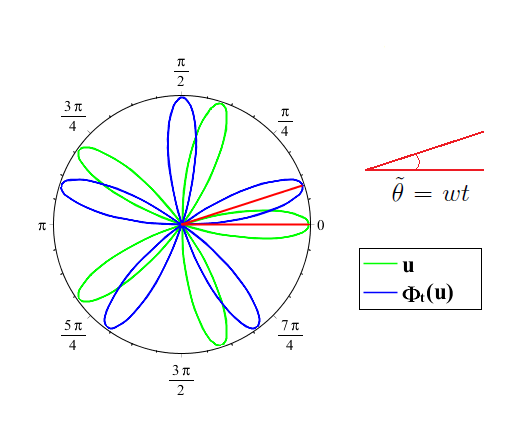
\includegraphics[height=8cm,keepaspectratio]{./figures/Pictures/rel_equi.png}}
\caption{The approach implemented to compute the rotating waves flow as a fixed point of the map $\Phi_{\tau}$. These fixed points of the map correspond to limit cycles of the continuous dynamical system. In particular, this approach can be used for system that admit $SO(2)$ symmetry.}
\label{rel_equ_fig}
%[Illustration of the implemented approach for the computation of the rotating waves flow]
\end{figure}
Therefore, if we can find such an initial condition and an $w$ such that $\tilde{\theta} = wt$, then we have found a rotating wave. An illustration of this computation is shown in Figure~\ref{rel_equ_fig}. The limit cycle corresponding to the rotating wave can then be found from
\begin{align}
\label{rel_eqi_1}
\Phi_t(\mathbf{u},\mu) - \gamma\mathbf{u} = 0,
\end{align}
where the rotation operator $\gamma \in SO(2)$ acts on $\mathbf{u}$ via $\gamma\mathbf{u} = \mathbf{u}(r,\theta-\tilde{\theta})$.
Equation~(\ref{rel_eqi_1}) involves the unknown phase speed $w$ at which the waves rotate with an angle $\tilde{\theta} = wt$ after a time $t$. To obtain closure and uniqueness of~(\ref{rel_eqi_1}), we seek a solution that is orthogonal to the plane tangential to the symmetry generator $\pderiv{}{\theta}\mathbf{u}$, the derivative of $\mathbf{u}$ with respect to $\theta$. Therefore, we choose the extra equation to be
\begin{align}
\label{rel_eqi_2}
\pderiv{}{\theta}\mathbf{u}^{(0)}\cdot\left(\mathbf{u} - \mathbf{u}^{(0)} \right) = 0,
\end{align}
to close the system of equations, where $\mathbf{u}^{(0)}$ is the initial guess of the nonlinear solver. We have chosen to seek corrections orthogonal to $\mathbf{u}^{(0)}$ instead of $\mathbf{u}$ to remove the complication of working with a nonlinear equation.

The nonlinear system given by~(\ref{rel_eqi_1}) and~(\ref{rel_eqi_2}) can then be solved using the Newton-Raphson method, in which case the corrector step takes the form
\begin{subequations}\begin{align}
\label{lin_sys_limit_cycle}
\begin{bmatrix}
\textrm{D}_{\mathbf{u}} \Phi(\mathbf{u}_{j}^{(k)},\mu_j) - \gamma  & t\pderiv{\mathbf{u}_{j}^{(k)}}{\theta}\\
\pderiv{\mathbf{u}^{(0)}}{\theta}   & 0
\end{bmatrix}
\begin{bmatrix}
\delta \textbf{u}_j^{(k)}\\
\delta w_{j}^{(k)}
\end{bmatrix}
&=
\begin{bmatrix}
\mathbf{u}_{j}^{(k)}-\Phi(\mathbf{u}_j^{(k)},\mu_{j})  \\
\pderiv{\mathbf{u}^{(0)}}{\theta}\left(\mathbf{u}_{j}^{(k)} - \mathbf{u}^{(0)}\right)
\end{bmatrix},\\
\mathbf{u}_{j}^{(k+1)} &= \mathbf{u}_{j}^{(k)} + \delta\mathbf{u}_{j}^{(k)},\\
w_{j}^{(k+1)}& = w_{j}^{(k)} + \delta w_j^{(k)},
\end{align}\end{subequations}
where the subscript $j$ denotes the sequence of points on the solution curve, and the superscript $k$ denotes the Newton iteration.
This techniques represents an advantage over the standard approach discussed in Section~\ref{sc_st_ap} because the Jacobian matrix of the linear system is only of size ${(n+1)\times(n+1)}$, that is, only a single row and column larger than the Jacobian of the system for steady states. The system can also be computed using matrix-free methods as follows.
The action of the matrix in the upper left corner $\mathrm{D}_{\mathbf{u}}\Phi_{t}$ on the vector $\delta\mathbf{u}$ is approximated using the forward finite-difference shown previously~(\ref{for_fin_diff}).
%The unknown $\tau$ is included in the initial guess and is updated on each iteration.
The computation of the derivative with respect to the angle $\theta$ and the action of the rotation operator $\gamma$ on the vector $\delta\mathbf{u}$ are computed in spectral space as an element-wise multiplication using the Fast Fourier Transform (FFT).  As a result, the main cost in this computation is the time-integration. Using these techniques, the linear system~(\ref{lin_sys_limit_cycle}) is then solved using GMRES. Upon convergence to within a desired set tolerance to the limit cycle, its period $\tau$  is computed. This calculation is required for the linear stability analysis performed to identify the local behaviours of the limit cycles using time-integration method and is presented in Section~\ref{sec_lin_sta_ana}

\section{The Eigenvalue Problem}\label{sec_lin_sta_ana}
In this section, we discuss the linear stability analysis performed for the two types of fixed points computed, $(\mathbf{u},\mu)$ and $(\mathbf{u},w,\mu)$ of the flow maps $\Phi_{t}(\mathbf{u},\mu)$ and $\Phi_{\tau}(\mathbf{u},\mu)$  that correspond to steady states and limit cycles of the continuous dynamical system, respectively.
In practice, one would want to classify the parameter space into regions where the flow is \emph{asymptotically stable} or \emph{unstable}. In the annular electroconvection problem, we want to determine whether  small perturbations from an \emph{equilibrium} flow will grow, i.e. unstable, or will decay, i.e. linearly in time. The eigenvalues are a quantitative tool that can be used to divide the parameter space into regions of topological equivalence of the flow close to the fixed points. For maps, a fixed point is said to be \emph{linearly stable} if all eigenvalues of the Jacobian of the map lie in the unit circle of the complex plane, and \emph{unstable} if at least one eigenvalue lies outside the unit circle. Bifurcations of the system occur when an eigenvalue crosses the unit circle.
Generically, this can happen in three ways: 1) either a simple positive eigenvalue crosses the unit circle when $\lambda = 1$; this bifurcation is referred to as a fold bifurcation; or  2) a simple negative eigenvalue crosses the unit circle when $\lambda = -1$; this bifurcation is called a flip or period doubling bifurcation; or 3) a pair of complex conjugate eigenvalues crosses the unit circle when $\lambda_{1,2} = e^{\pm i\theta}, 0<\theta<\pi$; this bifurcation is called a Neimark-Sacker bifurcation~\cite{Kuznet}.

The eigenvalues of fixed points $(\mathbf{u}_i,\mu_i)$ of the flow maps can be obtained by solving
\begin{align}
\label{eig_prob}
\mathbf{Av} = \lambda\mathbf{v},
\end{align}
where $\mathbf{A} = \mathrm{D}_{\mathbf{u}}\Phi_t(\mathbf{u},\mu)$ in the case of fixed points corresponding to steady states and $\mathbf{A} = \mathrm{D}_{\mathbf{u}}\Phi_{\tau}(\mathbf{u},\mu)$ in the case of fixed points corresponding to limit cycles with period $\tau$. Note that $\mathrm{D}_{\mathbf{u}}\Phi_t(\mathbf{u},\mu)$ is the linearization of the map~(\ref{flow_map}) about fixed points $\mathbf{u}$. In practice, we do not want to compute all the eigenvalues of the system. In particular, we are only interested in the eigenvalues of largest modulus of $\mathbf{A}$.

In the case of the fixed point $(\mathbf{u},\mu)$, the action of the linearization $\mathrm{D}_{\mathbf{u}}\Phi_t(\mathbf{u},\mu)$ on the vector $\mathbf{v}$ can be approximated with~(\ref{for_fin_diff}) for arbitrary time $t$. This leads us to consider the Implicitly Restarted Arnoldi method (IRAM). Arnoldi methods are projection methods that construct an orthogonal basis of a Krylov subspace~\cite{tref_num_lin_alg}, and are efficient methods to reduce computation and storage requirements~\cite{eig_arpackusers}. The IRAM computes approximations of the eigenvalues of largest magnitude of a matrix using only matrix-vector products, and thus its implementation together with~(\ref{for_fin_diff}) leads to a matrix-free method. We use the IRAM MATLAB implementation \texttt{eigs}, which allows the matrix-vector product to be defined via a function rather than requiring the matrix to be defined explicitly.

As for the case of the fixed point $(\mathbf{u},\mu,w)$, the linearization about the solution requires the computation of the period $\tau$. This can be obtained by the relation between the period $\tau$ and the phase speed $w$ given by
\begin{align}
\label{period_comp}
w\tau = \frac{2\pi}{m},
\end{align}
where $m$ is the wave number of the rotating wave state. Upon computing the period, the action of the linearization of $\mathrm{D}_{\mathbf{u}}\Phi_\tau(\mathbf{u},\mu)$ is approximated with~(\ref{for_fin_diff}) and the ten eigenvalues with largest modulus are computed using \texttt{eigs}. By analyzing the eigenvalues, the local behaviour of the flow and bifurcations can be identified and characterized.


%The eigenvalues of (\ref{eig_prob}) can be approximated using matrix-free methods where the action of the Jacobian on the vector is approximated using  equation (\ref{for_fin_diff}). We use \texttt{eigs}, a MATLAB built-in function, which is an implementation of an implicit restarted Arnoldi method (IRAM). Arnoldi methods are projection methods that construct an orthogonal basis of a Krylov subspace \cite{tref_num_lin_alg}. This technique is introduced as an efficient method to reduce the computation and storage requirements \cite{eig_arpackusers}. For every solution point, the largest ten eigenvalues with their corresponding eigenvectors are computed.
%In the continuation methods, we traced two type of fixed points, one that corresponds to steady state solutions and one that corresponds to the limit cycle. Thus, To compute the stability of the fixed point corresponding to the steady state, the integration time can be in principle arbitrary, as for the fixed point corresponding to the limit cycle, the integration time is set to be the period of the limit cycle $\tau$ . The period is computed using the equation (\ref{period_comp}) upon converging to the fixed point corresponding to a limit cycle. If all eigenvalues lie inside the unit circle, the solution is linearly stable and the solution is unstable if at least one eigenvalue crosses the unit circle. We note that for the computation of the eigenvalues of the fixed point associated with the limit cycle, there exist a simple unity eigenvalue associated with the limit cycle.
